\section{Design-Based Results}
\label{sec:si_design_based}

This section presents additional results from the design-based Monte Carlo simulation that complement the main text findings.

\subsection{Relative Bias}
\label{sec:si_relative_bias}

Given that the study-period means are approximately normal in the two original full-year networks, neither estimator for the period mean is particularly biased. However, the daily mean lognormal estimator does demonstrate slightly more positive bias, as shown in Figure~\ref{fig:mrb_histograms}. Because we consider the unbiased reference mean as calculated as a function of the standard mean estimator, this result suggests that the lognormal estimator may generally be a more conservative estimate of \pmtt\, if we consider that the risk of overestimating mean air pollution exposure with respect to human health is less than the risk of underestimating. In the \city{Chicago} partial-year period Monte Carlo, the corresponding lognormal mean bias is much smaller (0.04--0.11\% across evaluated $n$), consistent with the narrower cross-sensor distributions visible in Figure~\ref{fig:si_daily_distributions}.

\begin{figure}[H]
 \centering
 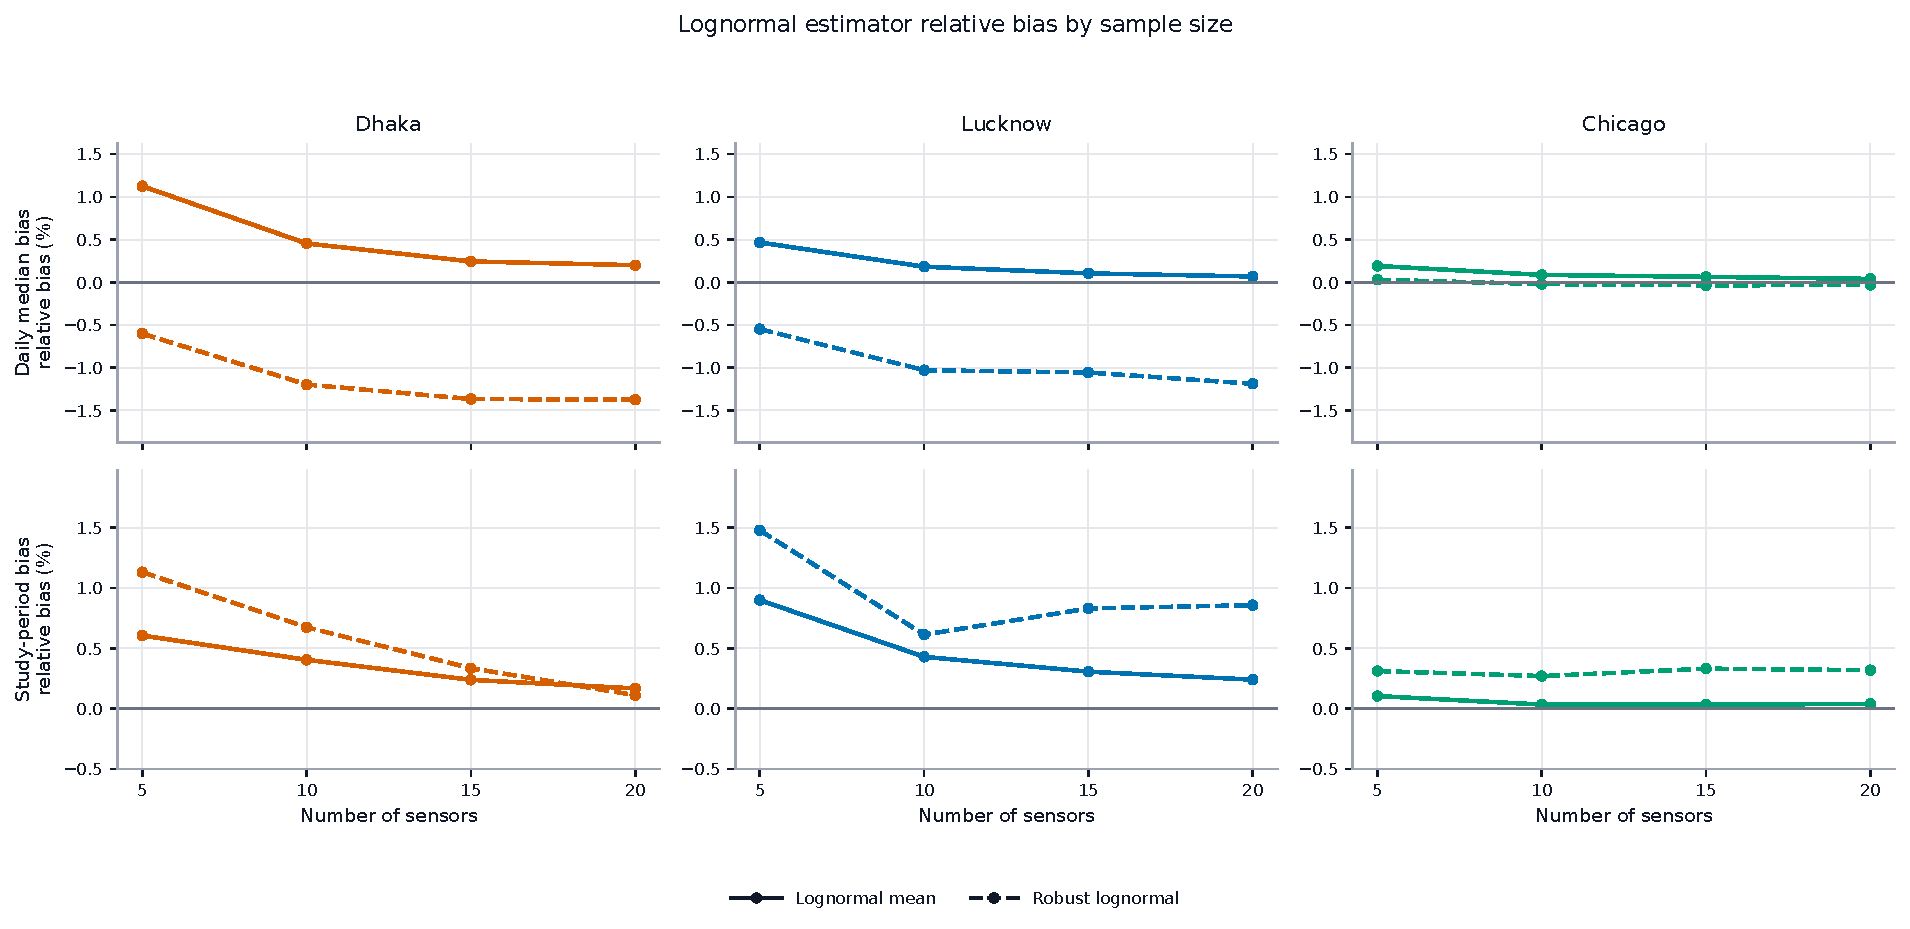
\includegraphics[width=0.95\textwidth]{Plots/Supporting_Information/Figure_SI_10/three_city_lognormal_relative_bias_by_n.pdf}
 \caption{Mean relative bias of the lognormal estimator as a function of subnetwork size $n$ for \city{Dhaka}, \city{Lucknow}, and \city{Chicago}. The bias is small in absolute terms in all three networks and tracks the cross-sensor skew (largest in \city{Lucknow}, smallest in \city{Chicago}). The \city{Chicago} curve covers the nine-month partial-year window.}
 \label{fig:mrb_histograms}
\end{figure}

\subsection{Quantile Coverage Error}
\label{sec:si_coverage}

As shown in Table~\ref{tab:ci} in the main text, the standard (arithmetic-mean, normal-theory) intervals are better calibrated than the lognormal intervals at the 68\% and 90\% levels across the sample sizes evaluated; the lognormal intervals are only marginally better at the 95\% level for the smallest $n$ and remain notably miscalibrated at the 68\% level. Coverage is nonetheless imperfect on some days for both estimators, even at sample sizes $>25$. This raises the question of optimal confidence interval estimation for air pollution data. We expect that alternative methods to the standard confidence interval technique used here may be more appropriate. However, we leave such exploration for future work.

\subsection{Worst-case subnetwork behavior: APE percentiles}\label{sec:si_worst_case}

While the main text reports MdAPE to characterize the \emph{typical} subnetwork error, network designers may equally care about how bad a suboptimal random subnetwork can be. We therefore report the median, 95th percentile, and observed maximum APE for each $n$ and each network across the $B = 10{,}000$ Monte Carlo draws. Table~\ref{tab:si_worst_case_period} summarizes the study-period results. The 95th-percentile APE remains noticeably above the median at small $n$ in all three networks (illustrating the right-skewed distribution of subnetwork errors), but converges toward the median by $n \approx 20$--$30$. For example, in \city{Lucknow} the 95th-percentile APE at $n=5$ is 23.2\% (median 8.0\%) and at $n=30$ falls to 7.5\% (median 2.6\%); in \city{Dhaka} the same percentiles fall from 17.3\% to 2.8\%; in \city{Chicago} from 9.1\% to 3.6\%.

\begin{table}[ht]
\centering
\small
\caption{Study-period APE percentiles across $B = 10{,}000$ SRSWOR draws for each city and subnetwork size. \emph{Median} is the typical subnetwork error (MdAPE); \emph{P95} characterizes the suboptimal-draw tail; \emph{worst} is the maximum observed APE across draws. Reference means: \city{Lucknow} 61.8~\units, \city{Dhaka} 55.1~\units, \city{Chicago} 10.3~\units.}
\label{tab:si_worst_case_period}
\begin{tabular}{lrrrrrrrrr}
\toprule
 & \multicolumn{3}{c}{\textbf{Lucknow}} & \multicolumn{3}{c}{\textbf{Dhaka}} & \multicolumn{3}{c}{\textbf{Chicago}} \\
\cmidrule(lr){2-4}\cmidrule(lr){5-7}\cmidrule(lr){8-10}
$n$ & Median & P95 & Worst & Median & P95 & Worst & Median & P95 & Worst \\
\midrule
5 & 8.0\% & 23.2\% & 54.7\% & 5.9\% & 17.3\% & 30.3\% & 2.6\% & 9.1\% & 25.7\% \\
10 & 5.6\% & 15.8\% & 30.1\% & 3.9\% & 10.9\% & 19.1\% & 1.9\% & 6.6\% & 16.8\% \\
20 & 3.6\% & 10.4\% & 20.9\% & 2.1\% & 5.9\% & 9.7\% & 1.4\% & 4.6\% & 9.1\% \\
30 & 2.6\% & 7.5\% & 15.0\% & 1.0\% & 2.8\% & 5.3\% & 1.2\% & 3.6\% & 7.7\% \\
\bottomrule
\end{tabular}
\end{table}

Figure~\ref{fig:si_period_error_bands} visualizes these results as relative-error and absolute-concentration percentile curves, making the right-skewed nature of the subnetwork-error distribution at small $n$ directly visible alongside the median curves used in the main text.

\begin{figure}[H]
 \centering
 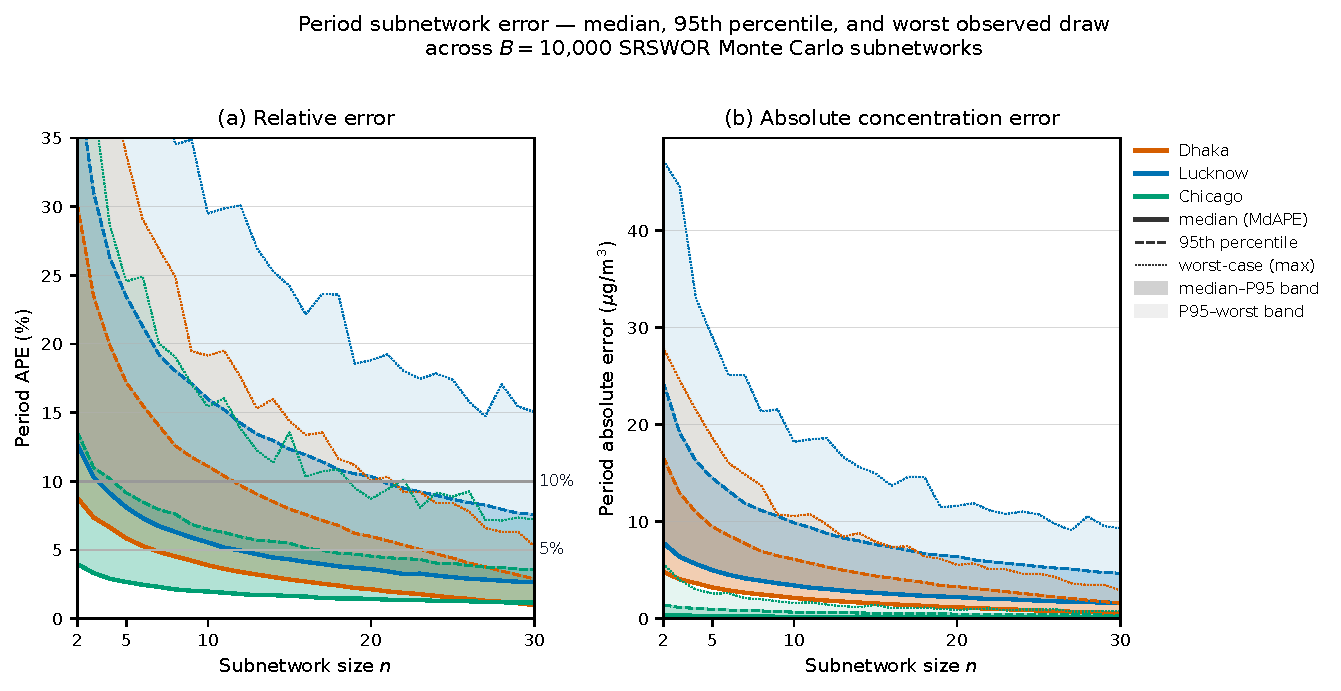
\includegraphics[width=0.98\textwidth]{Plots/Supporting_Information/Figure_SI_14/period_error_percentile_bands.pdf}
 \caption{Period subnetwork error vs subnetwork size $n$, characterizing both typical and worst-case behavior. (a) Relative error in percent. (b) Absolute concentration error in \units. For each city the solid line shows the median APE (MdAPE), the dashed line shows the 95th percentile across $B=10{,}000$ SRSWOR draws, and the dotted line shows the worst observed draw. Horizontal guides in (a) mark the 5\% and 10\% MdAPE thresholds. The figure shows that subnetwork error is markedly right-skewed at small $n$ (particularly in \city{Lucknow}), and that the absolute concentration error at any given $n$ differs by roughly an order of magnitude between \city{Chicago} and the South Asian networks despite their similar percentage-error curves at moderate $n$.}
 \label{fig:si_period_error_bands}
\end{figure}

The corresponding daily-MdAPE percentiles --- collapsed across days as the across-day median, 95th percentile, and worst single day --- show qualitatively similar convergence but with much heavier tails on the worst single day. For example, at $n=5$ the across-day median daily MdAPE is 6.5\% in \city{Lucknow}, but the worst single day (January~17, 2023) reaches 194\%; the worst \city{Dhaka} day at $n=5$ (February~10, 2023) reaches 127\%, and the worst \city{Chicago} day at $n=5$ (March~13, 2026) reaches 240\%. These extreme single days are concentrated in periods of high cross-sensor coefficient of variation (Section~\ref{sec:si_high_error_days}). Full curves for the period and daily cases, together with the underlying data, are provided in the released analysis outputs.

\subsection{Absolute concentration error}\label{sec:si_absolute_error}

Because percentage errors can obscure policy-relevant concentration errors, particularly across networks with markedly different baseline \pmtt\ levels, we provide absolute-concentration analogues of the main MdAPE curves in \units. The period and daily absolute-error curves are provided in the released analysis outputs. The absolute-error view makes the order-of-magnitude difference in baseline \pmtt\ between the South Asian networks ($\sim 50$--$100$~\units\ daily means in winter) and the Chicago network ($\sim 5$--$15$~\units) directly visible, and clarifies that a 5\%--10\% percentage error in Chicago corresponds to a much smaller absolute concentration error than the same percentage in \city{Dhaka} or \city{Lucknow}.

\subsection{High-error day characterization}\label{sec:si_high_error_days}

The main text notes that elevated daily MdAPE is associated with disproportionately high cross-sensor coefficient of variation rather than necessarily with elevated mean \pmtt. We characterized high-error days more formally using a regression and clustering analysis.

An ordinary least-squares model relating daily $n=10$ MdAPE to daily descriptors (cross-sensor spatial standard deviation, spatial coefficient of variation, missingness fraction, valid-sensor fraction, and \pmtt\ level) achieves $R^2 = 0.95$ in cross-validation (RMSE $= 0.50$ percentage points, MAE $= 0.29$), indicating that the broad error structure is highly predictable from observable daily descriptors. The corresponding in-sample $R^2$ is $0.95$ as well. The strongest correlates of daily MdAPE are the daily spatial standard deviation and the daily spatial coefficient of variation, with the daily missingness fraction also contributing; \pmtt\ level itself is a much weaker correlate. The corresponding model for study-period MdAPE achieves $R^2 = 0.72$ in cross-validation (RMSE $= 0.88$ percentage points), with the sensor-count curve being the dominant predictor and city as a secondary factor.

K-means clustering of the daily descriptor profiles separates the three cities almost perfectly (city-majority cluster accuracy $= 0.97$), meaning that day-level profiles are city-specific even before considering error. Per-city clustering (with $k=4$ chosen by silhouette in each city) identifies a small ``high-spatial-heterogeneity'' cluster in each city that contributes disproportionately to the tails of the APE distribution; the worst single days listed in Section~\ref{sec:si_worst_case} all sit within this cluster. Sensor-level clustering (with $k=2$ optimal in each city by silhouette: 0.58, 0.29, 0.31 for \city{Chicago}, \city{Dhaka}, \city{Lucknow} respectively) identifies a small number of sensors that are over-represented on high-error days, although no single sensor is responsible for a large fraction of those days. Full cluster assignments, sensor membership, high-error-day timestamps, and the high-error-day visualization are provided in the released analysis outputs.

\subsection{Cross-sensor heterogeneity and subnetwork error}\label{sec:si_cv_slope}

As an interpretable complement to the multivariable model above, we report the per-city slope of daily MdAPE at $n=10$ regressed on the daily cross-sensor coefficient of variation. The slope is a single-number summary of how strongly day-to-day cross-sensor heterogeneity translates into subnetwork error, separately for each city. Source data are in the released analysis outputs.

Across the three networks, the slopes are distinct and the $95\%$ confidence intervals do not overlap: \city{Dhaka} $\beta=0.203$ (CI $0.199$, $0.206$), $R^2=0.97$, $365$ days; \city{Lucknow} $\beta=0.156$ (CI $0.153$, $0.159$), $R^2=0.96$, $365$ days; \city{Chicago} $\beta=0.108$ (CI $0.099$, $0.118$), $R^2=0.63$, $272$ days. At matched cross-sensor heterogeneity, the South Asian networks therefore translate that heterogeneity into subnetwork error roughly twice as steeply as the \city{Chicago} network. Figure~\ref{fig:si_cv_slope} shows the three-city scatter with fits and shaded $95\%$ confidence bands.

\begin{figure}[H]
 \centering
 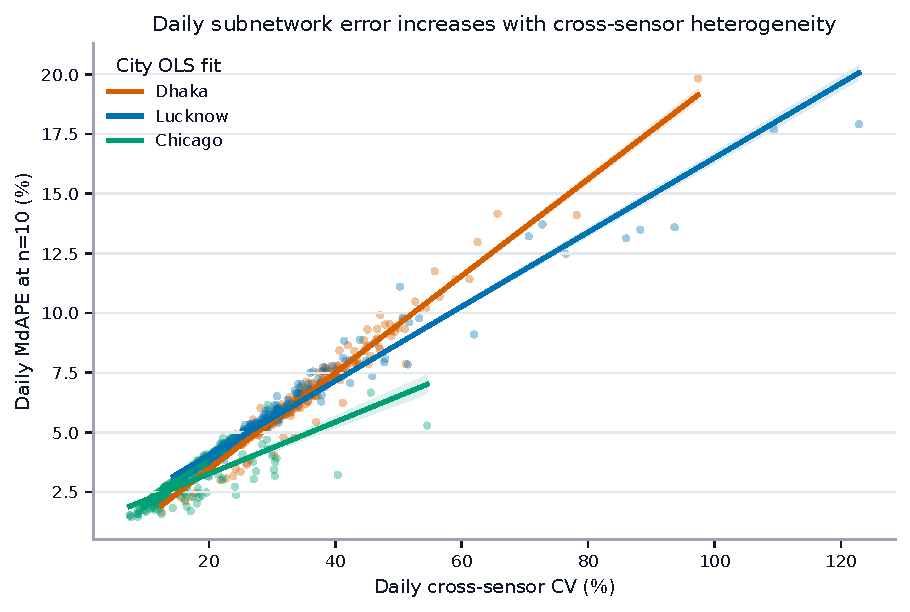
\includegraphics[width=0.7\textwidth]{Plots/Supporting_Information/Figure_SI_20/three_city_mdape_vs_cv_slope.pdf}
 \caption{Daily $n=10$ MdAPE vs.\ daily cross-sensor coefficient of variation, with city-specific ordinary-least-squares fits and shaded $95\%$ confidence bands. Per-city slopes (with non-overlapping $95\%$ confidence intervals) quantify how strongly cross-sensor heterogeneity translates into subnetwork error in each network: $\beta_{\mathrm{Dhaka}}=0.203$, $\beta_{\mathrm{Lucknow}}=0.156$, $\beta_{\mathrm{Chicago}}=0.108$.}
 \label{fig:si_cv_slope}
\end{figure}

The interpretation we adopt for the slope is deliberately narrow: it is the rate at which day-to-day spatial heterogeneity is reflected in subnetwork error, conditional on the network, not a formal variance decomposition into ``local sources'' versus other components. A clean variance decomposition would require additional model structure that we did not validate.

\subsection{Seasonal and monthly subnetwork convergence}\label{sec:si_seasonal_convergence}

Because annual convergence with very few sensors may partly reflect regionally coherent seasonal patterns, we additionally report subnetwork convergence stratified by month and by season. Monthly summaries are in the released analysis outputs. At $n=10$, the median monthly MdAPE is 4.9\% in \city{Dhaka} (with a maximum of 7.6\% in March 2023), 4.8\% in \city{Lucknow} (max 6.9\% in January 2023), and 2.1\% in \city{Chicago} (max 2.5\% in January 2026). The worst-performing months in the South Asian networks are the high-pollution winter months (Lucknow January 2023 with reference mean $148~\units$, Dhaka November 2022 and March 2023), but the cross-month range of MdAPE is modest --- a factor of roughly 1.5 between best and worst months rather than an order of magnitude. The seasonal aggregation (winter / pre-monsoon / monsoon / post-monsoon, where applicable) shows the same pattern more compactly: at $n=10$ the seasonal-median MdAPE is 4.3\% in \city{Dhaka}, 4.7\% in \city{Lucknow}, and 2.1\% in \city{Chicago}, with seasonal maxima 5.1\%, 6.1\%, and 2.4\% respectively. This is consistent with the interpretation that the all-year sensor-count recommendation is reasonable across seasons rather than being driven primarily by a single low-variance season, although winter peaks do increase the required sensor count modestly.

\subsection{Chicago daily subnetwork behavior}\label{sec:si_chicago_daily}

For completeness, we include daily MdAPE figures for the \city{Chicago} partial-year window, plotted in the same format as Figure~3 of the main text but with the secondary axis showing the daily count of valid Chicago sensors $N^*$. These figures are in the released analysis outputs. Chicago's much larger $N$ keeps even $n=20$ draws far from the available population on every day, and the daily MdAPE curve sits below the South Asian curves on most days, consistent with the lower coefficient of variation across the Chicago network.
